%==========================================================================
%==========================================================================
%
% Vzorovy text EXAMPKCSF.TEX v LATEX2e
%
%==========================================================================
%
%\documentstyle[a4]{article}
\documentclass[twoside]{articlek}
\newcommand{\mins}{&\!\!\!\!}
\renewcommand{\refname}{REFERENCES}
\textwidth=17.3truecm \hoffset=0.55truecm \textheight=26.4truecm
\topmargin=-2.2truecm \columnsep=0.7truecm \oddsidemargin =
-.4truecm \evensidemargin = -1.7truecm \pagenumbering{arabic}
\pagestyle{headings} \setcounter{page}{0}
\newlength{\sectionName}
\newlength{\sectionNameP}
\unitlength=1cm
\frenchspacing
%\parindent=0cm
\def\be{\begin{equation}}
\def\ee{\end{equation}}
% ------------------------------------------------------------------------

\def\BibTeX{{\rm B\kern-.05em{\sc i\kern-.025em b}\kern-.08em
            T\kern-.1667em\lower.7ex\hbox{E}\kern-.125emX}}

\usepackage{graphicx}
% ------------------------------------------------------------------------
\begin{document}
\sloppy
\twocolumn[{
%\vspace*{1.7cm}   % for the title  page only
%\begin{center}
{\large\bf INSTRUCTIONS FOR AUTHORS}\\

{\small A. Author, e-mail, B. Author, e-mail, address and C.
Author, e-mail, address}\\

%\end{center}
%\vspace*{1ex}

%{\bf ABSTRACT.} These are the guidelines for preparation of
%manuscripts of the contributions to the proceedings of the 17th
%Conference of Czech and Slovak Physicists, held on September 5 -
%8, 2011.\\
}]
%---------------------------------------------------------------------------
\section{INTRODUCTION}

All manuscripts should be written in good English. It is very
important that your final paper should have the right number of
pages: two for contributed and six pages for invited papers,
including figures and
tables. This example file help you to prepare contribution in a
form of camera ready.

Send your manuscript by e-mail as file with name "AUTHOR.tex"
(AUTHOR = your name) written in LaTeX2e together with all figures
in EPS format.

\section{SECTION}

The section titles are written in bold capitals. The equations are
written and numbered as following example.

\be
s = at^2/2.
\ee

Due to two columns style please use the figure and table width up
to 8 cm preferentially.

%FIG 1
%
\begin{figure} [h,t]                     %instead of \begin{figure}[t]
\begin{center}                        %instead of \begin{center}
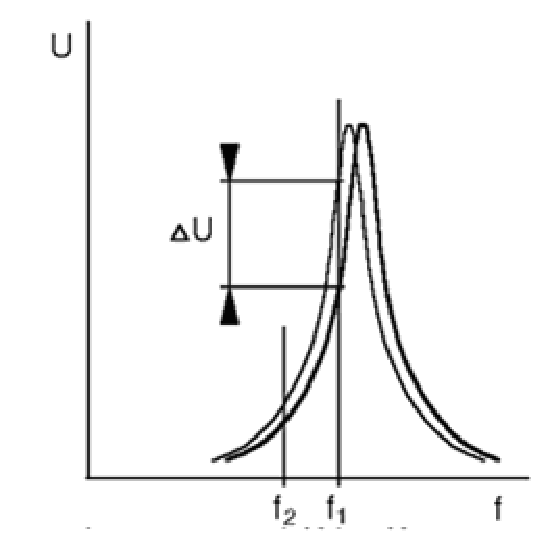
\includegraphics[width=80mm]{fig1.eps}   % for LaTeX 2e
%\epsfig{file=1a.eps, width=80mm, height=60mm, clip=} % for LaTeX 2.09
\end{center}                         %instead of \end{center}
\vspace{-2mm} \caption{This is figure caption.}
\end{figure}                        %instead of \end{figure}

You should layout your figures in the EPS graphic format without
preview.

Each table should include the above heading with description of
the content of the table.

\begin{table}[ht]
\begin{center}
 \caption{This is figure caption.}
\begin{tabular}{|l|r|r|}
\hline
J\'{a}n Poliak\hbox{\hspace{.5cm}}&\hbox{\hspace{1.5cm}}10.13&\hbox{\hspace{1.5cm}}25.26\\
\hline
Peter \v{C}ech&11.03&26.25\\
\hline
Jozef Slov\'{a}k&10.31&25.62\\
\hline
\end{tabular}
\end{center}
\end{table}


The references within the text should be referred to with
consecutive numbers in square brackets or you can use TeX command
\cite{RA_82}. Each your contribution should be the presentation of
news in physics and in your field during last time. All
interesting people could contact you by e-mail.

\section{CONCLUSIONS}

The manuscripts have to be send up to 30.~08.~2011 by e-mail to
address: reiffers@saske.sk\\

\noindent ACKNOWLEDGMENT: This example will be prepared to
download under file name "exampkcsf.zip" in address
"http://sfs.sav.sk".\\
%\renewcommand{\section}[1]{}

\begin{thebibliography}{99}

%\newcommand{\noopsort}[1]{} \newcommand{\printfirst}[2]{#1}
%      \newcommand{\singleletter}[1]{#1} \newcommand{\switchargs}[2]{#2#1}
\leftskip=-5pt \vspace{-0.3truecm}
\bibitem{RA_82} R.~Autor, Journal a. {\bf 2}, 2345 (2001).
\bibitem{SA_77} S.~Autor, Journal b. {\bf 32}, 4567 (2002).
\bibitem{4} B. Author: Book name (Publisher, town - 2003).
\end{thebibliography}

\end{document}
